\documentclass[10pt]{article}
%% fitch.sty
%% Macros for Fitch-style natural deduction
%% Copyright 2002-2023 Peter Selinger
%
% This work may be distributed and/or modified under the
% conditions of the LaTeX Project Public License, either version 1.3
% of this license or (at your option) any later version.
% The latest version of this license is in
%   https://www.latex-project.org/lppl.txt
% and version 1.3c or later is part of all distributions of LaTeX
% version 2008 or later.
%
% This work has the LPPL maintenance status `maintained'.
% 
% The Current Maintainer of this work is Richard Zach <rzach@ucalgary.ca>
%
% This work consists of the files fitch.sty and fitchdoc.tex.

% Original Author: Peter Selinger, Dalhousie University
% Created: Jan 14, 2002
% Modified: December 17, 2023
% Version: 1.0
% Copyright: (C) 2002-2005 Peter Selinger, Richard Zach
% Filename: fitch.sty
% Documentation: fitchdoc.tex
% https://github.com/OpenLogicProject/fitch/

% USAGE EXAMPLE:
% 
% The following is a simple example illustrating the usage of this
% package.  For detailed instructions and additional functionality, see
% the user guide, which can be found in the file fitchdoc.tex.
% 
% \[
% \begin{nd}
%   \hypo{1}  {P\vee Q}   
%   \hypo{2}  {\neg Q}                         
%   \open                              
%   \hypo{3a} {P}
%   \have{3b} {P}        \r{3a}
%   \close                   
%   \open
%   \hypo{4a} {Q}
%   \have{4b} {\neg Q}   \r{2}
%   \have{4c} {\bot}     \ne{4a,4b}
%   \have{4d} {P}        \be{4c}
%   \close                             
%   \have{5}  {P}        \oe{1,3a-3b,4a-4d}                 
% \end{nd}
% \]

\NeedsTeXFormat{LaTeX2e}
\ProvidesPackage{fitch}[2023-12-17 v1.0 Macros for Fitch-style natural deduction]

% Define keyval options

\RequirePackage{kvoptions}

\SetupKeyvalOptions{
family = fitch,
prefix = nd@ % prefix with nd@ for compatibility with old code
}

\DeclareStringOption[ndrules]{rules}
\DeclareStringOption[array]{arrayenv}
\DeclareStringOption[ndjustformat]{justformat}
\DeclareStringOption[ndrefformat]{refformat}

\DeclareStringOption[4.5ex]{height}[4.5ex]
\DeclareStringOption[3.5ex]{topheight}[3.5ex]
\DeclareStringOption[1.5ex]{depth}[1.5ex]
\DeclareStringOption[1em]{labelsep}[1em]
\DeclareStringOption[1.6em]{indent}[1.6em]
\DeclareStringOption[1.5ex]{hsep}[1.5ex]
\DeclareStringOption[2.5em]{justsep}[2.5em]
\DeclareStringOption[.2mm]{linethickness}[.2mm]
\DeclareStringOption[1em]{cindent}[1em]
\DeclareBoolOption[true]{outerline}

% user command to redefine dimensions
\def\nddim#1#2#3#4#5#6#7#8{
  \setkeys{fitch}{
    height=#1,
    topheight=#2,
    depth=#3,
    labelsep=#4,
    indent=#5,
    hsep=#6,
    justsep=#7,
    linethickness=#8
  }
}

\DeclareLocalOptions{
  rules,
  arrayenv,
  justformat,
  refformat,
  height,
  topheight,
  depth,
  labelsep,
  indent,
  hsep,
  justsep,
  linethickness,
  cindent,
  outerline
}

\ProcessLocalKeyvalOptions{fitch}

% Actual fitch.sty code

\newlength{\nd@dim}

% References

\newcount\nd@ctr
\def\nd@render{\expandafter\ifx\expandafter\nd@x\nd@base\nd@x\the\nd@ctr\else\nd@base\ifnum\nd@ctr<0\the\nd@ctr\else\ifnum\nd@ctr>0+\the\nd@ctr\fi\fi\fi}
\expandafter\def\csname nd@-\endcsname{}

\def\nd@num#1{\nd@numo{\nd@render}{#1}\global\advance\nd@ctr1}
\def\nd@numopt#1#2{\nd@numo{$#1$}{#2}}
\def\nd@numo#1#2{\edef\x{#1}\mbox{$\x$}\expandafter\global\expandafter\let\csname nd@-#2\endcsname\x}
\def\nd@ref#1{\expandafter\let\expandafter\x\csname nd@-#1\endcsname\ifx\x\relax%
  \PackageWarning{fitch}{Undefined line reference: #1}\mbox{\textbf{??}}\else\csname\nd@refformat\endcsname{\mbox{$\x$}}\fi}
\def\nd@noop{}
\def\nd@set#1#2{\ifx\relax#1\nd@noop\else\global\def\nd@base{#1}\fi\ifx\relax#2\relax\else\global\nd@ctr=#2\fi}
\def\nd@reset{\nd@set{}{1}}
\def\nd@refa#1{\nd@ref{#1}}
\def\nd@aux#1#2{\ifx#2-\nd@refa{#1}--\def\nd@c{\nd@aux{}}%
  \else\ifx#2,\nd@refa{#1}, \def\nd@c{\nd@aux{}}%
  \else\ifx#2;\nd@refa{#1}; \def\nd@c{\nd@aux{}}%
  \else\ifx#2.\nd@refa{#1}. \def\nd@c{\nd@aux{}}%
  \else\ifx#2)\nd@refa{#1})\def\nd@c{\nd@aux{}}%
  \else\ifx#2(\nd@refa{#1}(\def\nd@c{\nd@aux{}}%
  \else\ifx#2\nd@end\nd@refa{#1}\def\nd@c{}%
  \else\def\nd@c{\nd@aux{#1#2}}%
  \fi\fi\fi\fi\fi\fi\fi\nd@c}
\def\ndref#1{\nd@aux{}#1\nd@end}

% Layer A

% set initial dimensions
%\nddim{4.5ex}{3.5ex}{1.5ex}{1em}{1.6em}{.5em}{2.5em}{.2mm}

\def\nd@v{\rule[-\nd@depth]{\nd@linethickness}{\nd@height}}
\def\nd@h{\rule[-\nd@depth]{0mm}{\nd@height}} % strut
\def\nd@t{\rule[-\nd@depth]{\nd@linethickness}{\nd@topheight}}
\def\nd@i{\hspace{\nd@indent}} 
\def\nd@s{\hspace{\nd@hsep}}
\def\nd@g#1{\nd@f{\makebox[\nd@indent][c]{$#1$}}}
\def\nd@f#1{\raisebox{0pt}[0pt][0pt]{$#1$}}
\def\nd@u#1{\makebox[0pt][l]{\settowidth{\nd@dim}{\nd@f{#1}}%
  \addtolength{\nd@dim}{\nd@hsep}\addtolength{\nd@dim}{\nd@hsep}%
  \hspace{-\nd@hsep}\rule[-\nd@depth]{\nd@dim}{\nd@linethickness}}\nd@f{#1}}

% Lists

\def\nd@push#1#2{\expandafter\gdef\expandafter#1\expandafter%
  {\expandafter\nd@cons\expandafter{#1}{#2}}}
\def\nd@pop#1{{\def\nd@nil{\gdef#1{\nd@nil}}\def\nd@cons##1##2%
    {\gdef#1{##1}}#1}}
\def\nd@iter#1#2{{\def\nd@nil{}\def\nd@cons##1##2{##1#2{##2}}#1}}
\def\nd@modify#1#2#3{{\def\nd@nil{\gdef#1{\nd@nil}}\def\nd@cons##1##2%
    {\advance#2-1 ##1\advance#2 1 \ifnum#2=1\nd@push#1{#3}\else%
      \nd@push#1{##2}\fi}#1}}

\def\nd@cont#1{{\def\nd@t{\nd@v}\def\nd@v{\nd@v}\def\nd@g##1{\nd@i}%
    \def\nd@i{\nd@i}\def\nd@nil{\gdef#1{\nd@nil}}\def\nd@cons##1##2%
    {##1\expandafter\nd@push\expandafter#1\expandafter{##2}}#1}}

% Layer B

\newcount\nd@n
\def\nd@beginb{%
  \begingroup
  \nd@reset
  \gdef\nd@stack{\nd@nil}%
  \nd@push\nd@stack{\nd@h}%
  \ifnd@outerline
    \nd@push\nd@stack{\nd@t}\fi
  \begin{\nd@arrayenv}{l@{\hspace{\nd@labelsep}}l@{\hspace{\nd@justsep}}l}}
\def\nd@resumeb{%
  \begingroup
  \begin{\nd@arrayenv}{l@{\hspace{\nd@labelsep}}l@{\hspace{\nd@justsep}}l}}
\def\nd@endb{\end{\nd@arrayenv}\endgroup}
\def\nd@hypob#1#2{\nd@f{\nd@num{#1}}&\nd@iter\nd@stack\relax\nd@cont\nd@stack\nd@s\nd@u{#2}&}
\def\nd@haveb#1#2{\nd@f{\nd@num{#1}}&\nd@iter\nd@stack\relax\nd@cont\nd@stack\nd@s\nd@f{#2}&}
\def\nd@havecontb#1#2{&\nd@iter\nd@stack\relax\nd@cont\nd@stack\nd@s\nd@f{\hspace{\nd@cindent}#2}&}
\def\nd@hypocontb#1#2{&\nd@iter\nd@stack\relax\nd@cont\nd@stack\nd@s\nd@u{\hspace{\nd@cindent}#2}&}

\def\nd@openb{\nd@push\nd@stack{\nd@i}\nd@push\nd@stack{\nd@t}}
\def\nd@closeb{\nd@pop\nd@stack\nd@pop\nd@stack}
\def\nd@guardb#1#2{\nd@n=#1\multiply\nd@n by 2 \nd@modify\nd@stack\nd@n{\nd@g{#2}}}

% Layer C

\def\nd@clr{\gdef\nd@cmd{}\gdef\nd@typ{\relax}}
\def\nd@sto#1#2#3{\gdef\nd@typ{#1}\gdef\nd@byt{}%
  \gdef\nd@cmd{\nd@typ{#2}{#3}\nd@byt\\}}
\def\nd@chtyp{\expandafter\ifx\nd@typ\nd@hypocontb\def\nd@typ{\nd@havecontb}\else\def\nd@typ{\nd@haveb}\fi}
\def\nd@hypoc#1#2{\nd@chtyp\nd@cmd\nd@sto{\nd@hypob}{#1}{#2}}
\def\nd@havec#1#2{\nd@cmd\nd@sto{\nd@haveb}{#1}{#2}}
\def\nd@hypocontc#1{\nd@chtyp\nd@cmd\nd@sto{\nd@hypocontb}{}{#1}}
\def\nd@havecontc#1{\nd@cmd\nd@sto{\nd@havecontb}{}{#1}}
\def\nd@by#1#2{\ifx\nd@x#2\nd@x\gdef\nd@byt{\mbox{#1}}\else\ifx\nd@x#1\nd@x\gdef\nd@byt{\mbox{\ndref{#2}}}\else\gdef\nd@byt{\mbox{\csname\nd@justformat\endcsname{#1}{\ndref{#2}}}}\fi\fi\ignorespaces}

% multi-line macros
\def\nd@mhypoc#1#2{\nd@mhypocA{#1}#2\\\nd@stop\\}
\def\nd@mhypocA#1#2\\{\nd@hypoc{#1}{#2}\nd@mhypocB}
\def\nd@mhypocB#1\\{\ifx\nd@stop#1\else\nd@hypocontc{#1}\expandafter\nd@mhypocB\fi}
\def\nd@mhavec#1#2{\nd@mhavecA{#1}#2\\\nd@stop\\}
\def\nd@mhavecA#1#2\\{\nd@havec{#1}{#2}\nd@mhavecB}
\def\nd@mhavecB#1\\{\ifx\nd@stop#1\else\nd@havecontc{#1}\expandafter\nd@mhavecB\fi}
\def\nd@mhypocontc#1{\nd@mhypocB#1\\\nd@stop\\}
\def\nd@mhavecontc#1{\nd@mhavecB#1\\\nd@stop\\}

\def\nd@beginc{\nd@beginb\nd@clr}
\def\nd@resumec{\nd@resumeb\nd@clr}
\def\nd@endc{\nd@cmd\nd@endb}
\def\nd@openc{\nd@cmd\nd@clr\nd@openb}
\def\nd@closec{\nd@cmd\nd@clr\nd@closeb}
\let\nd@guardc\nd@guardb

% Layer D

% macros with optional arguments spelled-out
\def\nd@hypod[#1][#2]#3[#4]#5{\ifx\relax#4\relax\else\nd@guardb{1}{#4}\fi\nd@mhypoc{#3}{#5}\nd@set{#1}{#2}\ignorespaces}
\def\nd@haved[#1][#2]#3[#4]#5{\ifx\relax#4\relax\else\nd@guardb{1}{#4}\fi\nd@mhavec{#3}{#5}\nd@set{#1}{#2}\ignorespaces}
\def\nd@havecont#1{\nd@mhavecontc{#1}}
\def\nd@hypocont#1{\nd@mhypocontc{#1}}
\def\nd@base{undefined}
\def\nd@opend[#1]#2{\nd@cmd\nd@clr\nd@openb\nd@guard{#1}#2}
\def\nd@close{\nd@cmd\nd@clr\nd@closeb}
\def\nd@guardd[#1]#2{\nd@guardb{#1}{#2}}

% Handling of optional arguments.

\def\nd@optarg#1#2#3{\ifx[#3\def\nd@c{#2#3}\else\def\nd@c{#2[#1]{#3}}\fi\nd@c}
\def\nd@optargg#1#2#3{\ifx[#3\def\nd@c{#1#3}\else\def\nd@c{#2{#3}}\fi\nd@c}

\def\nd@five#1{\nd@optargg{\nd@four{#1}}{\nd@two{#1}}}
\def\nd@four#1[#2]{\nd@optarg{0}{\nd@three{#1}[#2]}}
\def\nd@three#1[#2][#3]#4{\nd@optarg{}{#1[#2][#3]{#4}}}
\def\nd@two#1{\nd@three{#1}[\relax][]}

\def\nd@have{\nd@five{\nd@haved}}
\def\nd@hypo{\nd@five{\nd@hypod}}
\def\nd@open{\nd@optarg{}{\nd@opend}}
\def\nd@guard{\nd@optarg{1}{\nd@guardd}}

\def\nd@init{%
  \let\open\nd@open%
  \let\close\nd@close%
  \let\hypo\nd@hypo%
  \let\have\nd@have%
  \let\hypocont\nd@hypocont%
  \let\havecont\nd@havecont%
  \let\by\nd@by%
  \let\guard\nd@guard%
  \csname\nd@rules\endcsname
}

% Define default rule names

\def\ndrules{%
  \def\ii{\by{$\Rightarrow$I}}%
  \def\ie{\by{$\Rightarrow$E}}%
  \def\Ai{\by{$\forall$I}}%
  \def\Ae{\by{$\forall$E}}%
  \def\Ei{\by{$\exists$I}}%
  \def\Ee{\by{$\exists$E}}%
  \def\ai{\by{$\wedge$I}}%
  \def\ae{\by{$\wedge$E}}%
  \def\ai{\by{$\wedge$I}}%
  \def\ae{\by{$\wedge$E}}%
  \def\oi{\by{$\vee$I}}%
  \def\oe{\by{$\vee$E}}%
  \def\ni{\by{$\neg$I}}%
  \def\ne{\by{$\neg$E}}%
  \def\be{\by{$\bot$E}}%
  \def\nne{\by{$\neg\neg$E}}%
  \def\r{\by{R}}}

% default justification format

\newcommand{\ndjustformat}[2]{#1, #2}

% default line number format

\newcommand{\ndrefformat}[1]{#1}

% User-level commands for proofs

\newenvironment{nd}[1][]
  {\begingroup
  \setkeys{fitch}{#1}%
  \nd@init\nd@beginc\ignorespaces}
  {\nd@endc\endgroup}
\newenvironment{ndresume}[1][]
  {\begingroup
  \setkeys{fitch}{#1}%
  \nd@init\nd@resumec\ignorespaces}
  {\nd@endc\endgroup}
\newenvironment{fitchproof}[1][]
  {\begin{list}{}{\setlength{\leftmargin}{0pt}}\item\begin{nd}[#1]}
  {\end{nd}\end{list}}
\newenvironment{fitchproof*}[1][]
  {\begin{list}{}{\setlength{\leftmargin}{0pt}}\item\begin{ndresume}[#1]}
  {\end{ndresume}\end{list}}

% End of file fitch.sty


\usepackage{graphics}

\textwidth 6.5in \textheight 9.2in
\oddsidemargin 0in \topmargin 0in \headheight 0in \headsep -.25in

\parskip=1.1ex \parindent=0pt

\title{Fitch-style natural deduction macros}
\author{Peter Selinger\\University of Ottawa}
\date{Version 0.5, February 8, 2005}

\begin{document}
\maketitle

\section{Overview}

This document describes how to use the {\tt fitch.sty} macros for
typesetting Fitch-style natural deduction derivations. To load the macros,
simply put \verb!%% fitch.sty
%% Macros for Fitch-style natural deduction
%% Copyright 2002-2023 Peter Selinger
%
% This work may be distributed and/or modified under the
% conditions of the LaTeX Project Public License, either version 1.3
% of this license or (at your option) any later version.
% The latest version of this license is in
%   https://www.latex-project.org/lppl.txt
% and version 1.3c or later is part of all distributions of LaTeX
% version 2008 or later.
%
% This work has the LPPL maintenance status `maintained'.
% 
% The Current Maintainer of this work is Richard Zach <rzach@ucalgary.ca>
%
% This work consists of the files fitch.sty and fitchdoc.tex.

% Original Author: Peter Selinger, Dalhousie University
% Created: Jan 14, 2002
% Modified: December 17, 2023
% Version: 1.0
% Copyright: (C) 2002-2005 Peter Selinger, Richard Zach
% Filename: fitch.sty
% Documentation: fitchdoc.tex
% https://github.com/OpenLogicProject/fitch/

% USAGE EXAMPLE:
% 
% The following is a simple example illustrating the usage of this
% package.  For detailed instructions and additional functionality, see
% the user guide, which can be found in the file fitchdoc.tex.
% 
% \[
% \begin{nd}
%   \hypo{1}  {P\vee Q}   
%   \hypo{2}  {\neg Q}                         
%   \open                              
%   \hypo{3a} {P}
%   \have{3b} {P}        \r{3a}
%   \close                   
%   \open
%   \hypo{4a} {Q}
%   \have{4b} {\neg Q}   \r{2}
%   \have{4c} {\bot}     \ne{4a,4b}
%   \have{4d} {P}        \be{4c}
%   \close                             
%   \have{5}  {P}        \oe{1,3a-3b,4a-4d}                 
% \end{nd}
% \]

\NeedsTeXFormat{LaTeX2e}
\ProvidesPackage{fitch}[2023-12-17 v1.0 Macros for Fitch-style natural deduction]

% Define keyval options

\RequirePackage{kvoptions}

\SetupKeyvalOptions{
family = fitch,
prefix = nd@ % prefix with nd@ for compatibility with old code
}

\DeclareStringOption[ndrules]{rules}
\DeclareStringOption[array]{arrayenv}
\DeclareStringOption[ndjustformat]{justformat}
\DeclareStringOption[ndrefformat]{refformat}

\DeclareStringOption[4.5ex]{height}[4.5ex]
\DeclareStringOption[3.5ex]{topheight}[3.5ex]
\DeclareStringOption[1.5ex]{depth}[1.5ex]
\DeclareStringOption[1em]{labelsep}[1em]
\DeclareStringOption[1.6em]{indent}[1.6em]
\DeclareStringOption[1.5ex]{hsep}[1.5ex]
\DeclareStringOption[2.5em]{justsep}[2.5em]
\DeclareStringOption[.2mm]{linethickness}[.2mm]
\DeclareStringOption[1em]{cindent}[1em]
\DeclareBoolOption[true]{outerline}

% user command to redefine dimensions
\def\nddim#1#2#3#4#5#6#7#8{
  \setkeys{fitch}{
    height=#1,
    topheight=#2,
    depth=#3,
    labelsep=#4,
    indent=#5,
    hsep=#6,
    justsep=#7,
    linethickness=#8
  }
}

\DeclareLocalOptions{
  rules,
  arrayenv,
  justformat,
  refformat,
  height,
  topheight,
  depth,
  labelsep,
  indent,
  hsep,
  justsep,
  linethickness,
  cindent,
  outerline
}

\ProcessLocalKeyvalOptions{fitch}

% Actual fitch.sty code

\newlength{\nd@dim}

% References

\newcount\nd@ctr
\def\nd@render{\expandafter\ifx\expandafter\nd@x\nd@base\nd@x\the\nd@ctr\else\nd@base\ifnum\nd@ctr<0\the\nd@ctr\else\ifnum\nd@ctr>0+\the\nd@ctr\fi\fi\fi}
\expandafter\def\csname nd@-\endcsname{}

\def\nd@num#1{\nd@numo{\nd@render}{#1}\global\advance\nd@ctr1}
\def\nd@numopt#1#2{\nd@numo{$#1$}{#2}}
\def\nd@numo#1#2{\edef\x{#1}\mbox{$\x$}\expandafter\global\expandafter\let\csname nd@-#2\endcsname\x}
\def\nd@ref#1{\expandafter\let\expandafter\x\csname nd@-#1\endcsname\ifx\x\relax%
  \PackageWarning{fitch}{Undefined line reference: #1}\mbox{\textbf{??}}\else\csname\nd@refformat\endcsname{\mbox{$\x$}}\fi}
\def\nd@noop{}
\def\nd@set#1#2{\ifx\relax#1\nd@noop\else\global\def\nd@base{#1}\fi\ifx\relax#2\relax\else\global\nd@ctr=#2\fi}
\def\nd@reset{\nd@set{}{1}}
\def\nd@refa#1{\nd@ref{#1}}
\def\nd@aux#1#2{\ifx#2-\nd@refa{#1}--\def\nd@c{\nd@aux{}}%
  \else\ifx#2,\nd@refa{#1}, \def\nd@c{\nd@aux{}}%
  \else\ifx#2;\nd@refa{#1}; \def\nd@c{\nd@aux{}}%
  \else\ifx#2.\nd@refa{#1}. \def\nd@c{\nd@aux{}}%
  \else\ifx#2)\nd@refa{#1})\def\nd@c{\nd@aux{}}%
  \else\ifx#2(\nd@refa{#1}(\def\nd@c{\nd@aux{}}%
  \else\ifx#2\nd@end\nd@refa{#1}\def\nd@c{}%
  \else\def\nd@c{\nd@aux{#1#2}}%
  \fi\fi\fi\fi\fi\fi\fi\nd@c}
\def\ndref#1{\nd@aux{}#1\nd@end}

% Layer A

% set initial dimensions
%\nddim{4.5ex}{3.5ex}{1.5ex}{1em}{1.6em}{.5em}{2.5em}{.2mm}

\def\nd@v{\rule[-\nd@depth]{\nd@linethickness}{\nd@height}}
\def\nd@h{\rule[-\nd@depth]{0mm}{\nd@height}} % strut
\def\nd@t{\rule[-\nd@depth]{\nd@linethickness}{\nd@topheight}}
\def\nd@i{\hspace{\nd@indent}} 
\def\nd@s{\hspace{\nd@hsep}}
\def\nd@g#1{\nd@f{\makebox[\nd@indent][c]{$#1$}}}
\def\nd@f#1{\raisebox{0pt}[0pt][0pt]{$#1$}}
\def\nd@u#1{\makebox[0pt][l]{\settowidth{\nd@dim}{\nd@f{#1}}%
  \addtolength{\nd@dim}{\nd@hsep}\addtolength{\nd@dim}{\nd@hsep}%
  \hspace{-\nd@hsep}\rule[-\nd@depth]{\nd@dim}{\nd@linethickness}}\nd@f{#1}}

% Lists

\def\nd@push#1#2{\expandafter\gdef\expandafter#1\expandafter%
  {\expandafter\nd@cons\expandafter{#1}{#2}}}
\def\nd@pop#1{{\def\nd@nil{\gdef#1{\nd@nil}}\def\nd@cons##1##2%
    {\gdef#1{##1}}#1}}
\def\nd@iter#1#2{{\def\nd@nil{}\def\nd@cons##1##2{##1#2{##2}}#1}}
\def\nd@modify#1#2#3{{\def\nd@nil{\gdef#1{\nd@nil}}\def\nd@cons##1##2%
    {\advance#2-1 ##1\advance#2 1 \ifnum#2=1\nd@push#1{#3}\else%
      \nd@push#1{##2}\fi}#1}}

\def\nd@cont#1{{\def\nd@t{\nd@v}\def\nd@v{\nd@v}\def\nd@g##1{\nd@i}%
    \def\nd@i{\nd@i}\def\nd@nil{\gdef#1{\nd@nil}}\def\nd@cons##1##2%
    {##1\expandafter\nd@push\expandafter#1\expandafter{##2}}#1}}

% Layer B

\newcount\nd@n
\def\nd@beginb{%
  \begingroup
  \nd@reset
  \gdef\nd@stack{\nd@nil}%
  \nd@push\nd@stack{\nd@h}%
  \ifnd@outerline
    \nd@push\nd@stack{\nd@t}\fi
  \begin{\nd@arrayenv}{l@{\hspace{\nd@labelsep}}l@{\hspace{\nd@justsep}}l}}
\def\nd@resumeb{%
  \begingroup
  \begin{\nd@arrayenv}{l@{\hspace{\nd@labelsep}}l@{\hspace{\nd@justsep}}l}}
\def\nd@endb{\end{\nd@arrayenv}\endgroup}
\def\nd@hypob#1#2{\nd@f{\nd@num{#1}}&\nd@iter\nd@stack\relax\nd@cont\nd@stack\nd@s\nd@u{#2}&}
\def\nd@haveb#1#2{\nd@f{\nd@num{#1}}&\nd@iter\nd@stack\relax\nd@cont\nd@stack\nd@s\nd@f{#2}&}
\def\nd@havecontb#1#2{&\nd@iter\nd@stack\relax\nd@cont\nd@stack\nd@s\nd@f{\hspace{\nd@cindent}#2}&}
\def\nd@hypocontb#1#2{&\nd@iter\nd@stack\relax\nd@cont\nd@stack\nd@s\nd@u{\hspace{\nd@cindent}#2}&}

\def\nd@openb{\nd@push\nd@stack{\nd@i}\nd@push\nd@stack{\nd@t}}
\def\nd@closeb{\nd@pop\nd@stack\nd@pop\nd@stack}
\def\nd@guardb#1#2{\nd@n=#1\multiply\nd@n by 2 \nd@modify\nd@stack\nd@n{\nd@g{#2}}}

% Layer C

\def\nd@clr{\gdef\nd@cmd{}\gdef\nd@typ{\relax}}
\def\nd@sto#1#2#3{\gdef\nd@typ{#1}\gdef\nd@byt{}%
  \gdef\nd@cmd{\nd@typ{#2}{#3}\nd@byt\\}}
\def\nd@chtyp{\expandafter\ifx\nd@typ\nd@hypocontb\def\nd@typ{\nd@havecontb}\else\def\nd@typ{\nd@haveb}\fi}
\def\nd@hypoc#1#2{\nd@chtyp\nd@cmd\nd@sto{\nd@hypob}{#1}{#2}}
\def\nd@havec#1#2{\nd@cmd\nd@sto{\nd@haveb}{#1}{#2}}
\def\nd@hypocontc#1{\nd@chtyp\nd@cmd\nd@sto{\nd@hypocontb}{}{#1}}
\def\nd@havecontc#1{\nd@cmd\nd@sto{\nd@havecontb}{}{#1}}
\def\nd@by#1#2{\ifx\nd@x#2\nd@x\gdef\nd@byt{\mbox{#1}}\else\ifx\nd@x#1\nd@x\gdef\nd@byt{\mbox{\ndref{#2}}}\else\gdef\nd@byt{\mbox{\csname\nd@justformat\endcsname{#1}{\ndref{#2}}}}\fi\fi\ignorespaces}

% multi-line macros
\def\nd@mhypoc#1#2{\nd@mhypocA{#1}#2\\\nd@stop\\}
\def\nd@mhypocA#1#2\\{\nd@hypoc{#1}{#2}\nd@mhypocB}
\def\nd@mhypocB#1\\{\ifx\nd@stop#1\else\nd@hypocontc{#1}\expandafter\nd@mhypocB\fi}
\def\nd@mhavec#1#2{\nd@mhavecA{#1}#2\\\nd@stop\\}
\def\nd@mhavecA#1#2\\{\nd@havec{#1}{#2}\nd@mhavecB}
\def\nd@mhavecB#1\\{\ifx\nd@stop#1\else\nd@havecontc{#1}\expandafter\nd@mhavecB\fi}
\def\nd@mhypocontc#1{\nd@mhypocB#1\\\nd@stop\\}
\def\nd@mhavecontc#1{\nd@mhavecB#1\\\nd@stop\\}

\def\nd@beginc{\nd@beginb\nd@clr}
\def\nd@resumec{\nd@resumeb\nd@clr}
\def\nd@endc{\nd@cmd\nd@endb}
\def\nd@openc{\nd@cmd\nd@clr\nd@openb}
\def\nd@closec{\nd@cmd\nd@clr\nd@closeb}
\let\nd@guardc\nd@guardb

% Layer D

% macros with optional arguments spelled-out
\def\nd@hypod[#1][#2]#3[#4]#5{\ifx\relax#4\relax\else\nd@guardb{1}{#4}\fi\nd@mhypoc{#3}{#5}\nd@set{#1}{#2}\ignorespaces}
\def\nd@haved[#1][#2]#3[#4]#5{\ifx\relax#4\relax\else\nd@guardb{1}{#4}\fi\nd@mhavec{#3}{#5}\nd@set{#1}{#2}\ignorespaces}
\def\nd@havecont#1{\nd@mhavecontc{#1}}
\def\nd@hypocont#1{\nd@mhypocontc{#1}}
\def\nd@base{undefined}
\def\nd@opend[#1]#2{\nd@cmd\nd@clr\nd@openb\nd@guard{#1}#2}
\def\nd@close{\nd@cmd\nd@clr\nd@closeb}
\def\nd@guardd[#1]#2{\nd@guardb{#1}{#2}}

% Handling of optional arguments.

\def\nd@optarg#1#2#3{\ifx[#3\def\nd@c{#2#3}\else\def\nd@c{#2[#1]{#3}}\fi\nd@c}
\def\nd@optargg#1#2#3{\ifx[#3\def\nd@c{#1#3}\else\def\nd@c{#2{#3}}\fi\nd@c}

\def\nd@five#1{\nd@optargg{\nd@four{#1}}{\nd@two{#1}}}
\def\nd@four#1[#2]{\nd@optarg{0}{\nd@three{#1}[#2]}}
\def\nd@three#1[#2][#3]#4{\nd@optarg{}{#1[#2][#3]{#4}}}
\def\nd@two#1{\nd@three{#1}[\relax][]}

\def\nd@have{\nd@five{\nd@haved}}
\def\nd@hypo{\nd@five{\nd@hypod}}
\def\nd@open{\nd@optarg{}{\nd@opend}}
\def\nd@guard{\nd@optarg{1}{\nd@guardd}}

\def\nd@init{%
  \let\open\nd@open%
  \let\close\nd@close%
  \let\hypo\nd@hypo%
  \let\have\nd@have%
  \let\hypocont\nd@hypocont%
  \let\havecont\nd@havecont%
  \let\by\nd@by%
  \let\guard\nd@guard%
  \csname\nd@rules\endcsname
}

% Define default rule names

\def\ndrules{%
  \def\ii{\by{$\Rightarrow$I}}%
  \def\ie{\by{$\Rightarrow$E}}%
  \def\Ai{\by{$\forall$I}}%
  \def\Ae{\by{$\forall$E}}%
  \def\Ei{\by{$\exists$I}}%
  \def\Ee{\by{$\exists$E}}%
  \def\ai{\by{$\wedge$I}}%
  \def\ae{\by{$\wedge$E}}%
  \def\ai{\by{$\wedge$I}}%
  \def\ae{\by{$\wedge$E}}%
  \def\oi{\by{$\vee$I}}%
  \def\oe{\by{$\vee$E}}%
  \def\ni{\by{$\neg$I}}%
  \def\ne{\by{$\neg$E}}%
  \def\be{\by{$\bot$E}}%
  \def\nne{\by{$\neg\neg$E}}%
  \def\r{\by{R}}}

% default justification format

\newcommand{\ndjustformat}[2]{#1, #2}

% default line number format

\newcommand{\ndrefformat}[1]{#1}

% User-level commands for proofs

\newenvironment{nd}[1][]
  {\begingroup
  \setkeys{fitch}{#1}%
  \nd@init\nd@beginc\ignorespaces}
  {\nd@endc\endgroup}
\newenvironment{ndresume}[1][]
  {\begingroup
  \setkeys{fitch}{#1}%
  \nd@init\nd@resumec\ignorespaces}
  {\nd@endc\endgroup}
\newenvironment{fitchproof}[1][]
  {\begin{list}{}{\setlength{\leftmargin}{0pt}}\item\begin{nd}[#1]}
  {\end{nd}\end{list}}
\newenvironment{fitchproof*}[1][]
  {\begin{list}{}{\setlength{\leftmargin}{0pt}}\item\begin{ndresume}[#1]}
  {\end{ndresume}\end{list}}

% End of file fitch.sty

! near the beginning of your
{\LaTeX} file. 

Here is a natural deduction derivation, together with the code that
produced it:

\hfill
\begin{minipage}{2.5in}
$
\begin{nd}
  \hypo {1}  {P\vee Q}
  \hypo {2}  {\neg Q}
  \open
  \hypo {3} {P}
  \have {4} {P}        \r{3}
  \close
  \open
  \hypo {aa} {Q}
  \have {6} {\neg Q}   \r{2}
  \have {7} {\bot}     \ne{aa,6}
  \have {8} {P}        \be{7}
  \close
  \have {9} {P}        \oe{1,3-4,aa-8}
\end{nd}
$
\end{minipage}
\hfill
\begin{minipage}{3in}\small
\begin{verbatim}
\[
\begin{nd}
  \hypo {1}  {P\vee Q}
  \hypo {2}  {\neg Q}
  \open
  \hypo {3} {P}
  \have {4} {P}        \r{3}
  \close
  \open
  \hypo {aa} {Q}
  \have {6} {\neg Q}   \r{2}
  \have {7} {\bot}     \ne{aa,6}
  \have {8} {P}        \be{7}
  \close
  \have {9} {P}        \oe{1,3-4,aa-8}
\end{nd}
\]
\end{verbatim}
\end{minipage}
\hfill

A derivation consists of {\em lines}, and each line contains a {\em
  line number} and a {\em formula}. Some lines also carry a {\em
  justification}. Moreover, each line is either a {\em hypothesis} or
a {\em derived formula}. Generally, derived formulas carry a
justification, whereas hypotheses do not; however, the macros do not
enforce this.

Derivations are typeset inside the \verb!nd! environment, which must be
used in math mode. The commands \verb!\hypo! and \verb!\have! are used
to typeset one line of the derivation; \verb!\hypo! is used for
hypotheses, and \verb!\have! for derived formulas. Both commands take
a label and a formula as an argument. Note that the labels used to
identify lines in the derivation need not be actual line numbers; for
instance, in the above example, we used the label $aa$ instead of $5$.
In the output, lines are automatically numbered consecutively. Labels
may not contain any punctuation characters or spaces.

Subderivations are opened and closed with the commands \verb!\open! and
\verb!\close!. Finally, the following commands are provided for
annotating lines with justifications:

\hfill
\begin{tabular}{ll}
  \verb!\r!  & reiteration \\
  \verb!\ii! & implication introduction \\
  \verb!\ie! & implication elimination \\
  \verb!\ai! & and introduction \\
  \verb!\ae! & and elimination \\
\end{tabular} 
\hfill
\begin{tabular}{ll}
  \verb!\oi! & or introduction \\
  \verb!\oe! & or elimination \\
  \verb!\ni! & not introduction \\
  \verb!\ne! & not elimination \\
  \verb!\be! & bottom elimination \\
\end{tabular} 
\hfill
\begin{tabular}{ll}
  \verb!\nne! & double negation elimination \\
  \verb!\Ai! & forall introduction \\
  \verb!\Ae! & forall elimination \\
  \verb!\Ei! & exists introduction \\
  \verb!\Ee! & exists elimination \\
\end{tabular} 
\hfill~

Each such command takes a {\em reference list} as an argument. A
reference list is a string made from labels, commas, and hyphens, for
instance \verb!1,3a-3b,4a-4d!.

\section{Details}

\subsection{Guards}

Some natural deduction derivations with quantifiers use {\em guards}, as in
the following example:

\hfill
\begin{minipage}{2.5in}
$
\begin{nd}
  \hypo {1} {\exists x\forall y.P(x,y)}
  \open[v]
  \open[u]
  \hypo {2} {\forall y.P(u,y)}
  \have {3} {P(u,v)}                     \Ae{2}
  \have {4} {\exists x.P(x,v)}           \Ei{3}
  \close
  \have {5} {\exists x.P(x,v)}           \Ee{1,2-5}
  \close
  \have {6} {\forall y\exists x.P(x,y)}  \Ai{2-5}
\end{nd}
$
\end{minipage}
\hfill
\begin{minipage}{3.5in}\small
\begin{verbatim}
\[
\begin{nd}
  \hypo {1} {\exists x\forall y.P(x,y)}
  \open[v]
  \open[u]
  \hypo {2} {\forall y.P(u,y)}
  \have {3} {P(u,v)}                     \Ae{2}
  \have {4} {\exists x.P(x,v)}           \Ei{3}
  \close
  \have {5} {\exists x.P(x,v)}           \Ee{1,2-5}
  \close
  \have {6} {\forall y\exists x.P(x,y)}  \Ai{2-5}
\end{nd}
\]
\end{verbatim}
\end{minipage}

The guards $v$ and $u$ in line 2 were typeset by giving optional
arguments to the \verb!\open! commands of the respective
subderivations. 

For most purposes, the above way of specifying guards is sufficient.
However, there is another method, which allows a more flexible
placement of guards: before any line, you can give the command
\verb!\guard{u}! to add a guard $u$ to the top-level subderivation at
that line, or \verb!\guard[n]{u}! to add a guard to the $n$th
enclosing subderivation at that line. Thus, the above example could
have also been typeset by inserting the two commands \verb!\guard{u}! and
\verb!\guard[2]{v}! just after the second \verb!\open! statement.

% For backward compatibility, there is a third way of specifying guards
% by giving an optional second argument to the \verb!\hypo! and
% \verb!\have! commands. The use of this feature is discouraged.

\subsection{Generic justifications}

Non-standard justifications can be created with the \verb!\by!
command. This command takes two arguments: a name and a reference
list. For instance, the command \verb!\by{De Morgan}{lab3,lab4}! might
produce the output ``\mbox{De Morgan, 3, 4}''. Note that the justification
is typeset in text mode. A comma is automatically inserted between the
name and the reference list, unless the reference list is empty.

\subsection{Label and reference list details}

Labels may not contain commas, periods, semicolons, hyphens,
parenthesis, or spaces. In a reference list, spaces are ignored (even
within a label!), whereas commas, periods, semicolons, parenthesis,
and hyphens are copied to the output. All other characters are
interpreted as part of a label. Attempting to reference a label which
has not been previously defined by any \verb!\hypo! or \verb!\have!
command produces an error message of the form:

\begin{verbatim}
  ! Undefined natdeduction reference: lab17.
\end{verbatim}

\subsection{Referencing line numbers in the text}
\label{subsec-ndref}

Labels defined in an \verb!nd! environment can be referenced in the
text with the \verb!\ndref! command. This command takes a reference
list as an argument, and produces the corresponding output. However,
it is only possible to reference labels {\em after} the corresponding
derivation has been typeset. There is currently no convenient way of
defining forward references. Also, if a label is used more than once,
\verb!\ndref! will always refer to the most recent time it was used.

\subsection{Scope}

The commands \verb!\hypo!, \verb!\have!, \verb!\open!, \verb!\close!,
\verb!\r!, \verb!\ii!, and so forth are only available inside an
\verb!nd! environment. These commands may have a different meaning
elsewhere in the same document. The only commands provided by the
\verb!fitch.sty!  package which are visible outside an \verb!nd!
environment are the command \verb!\ndref! described in
Section~\ref{subsec-ndref}, and the command \verb!\nddim! and the
dimension \verb!\ndindent! described in Section~\ref{subsec-nddim}.

\subsection{Breaking it across pages}\label{subsec-break}

The \verb!nd! environment is derived from the {\LaTeX} \verb!array!
environment, and thus it does not break across pages automatically. 
However, if a derivation is too long to fit on a single page, it is
possible to split it manually into physically independent, but
logically consecutive subparts. For this purpose, the \verb!ndresume!
environment is provided to continue a previously interrupted
derivation. Here is an example:

\hfill
\begin{minipage}{2.5in}
$
\begin{nd}
  \hypo {1}  {P\vee Q}
  \hypo {2}  {\neg Q}
  \open
  \hypo {3} {P}
  \have {4} {P}        \r{3}
  \close
  \open
  \hypo {aa} {Q}
  \have {6} {\neg Q}   \r{2}
\end{nd}
$

Derivations can be interrupted and 
resumed at any point.

$
\begin{ndresume}
  \have {7} {\bot}     \ne{aa,6}
  \have {8} {P}        \be{7}
  \close
  \have {9} {P}        \oe{1,3-4,aa-8}
\end{ndresume}
$
\end{minipage}
\hfill
\begin{minipage}{3in}\small
\begin{verbatim}
$
\begin{nd}
  \hypo {1}  {P\vee Q}
  \hypo {2}  {\neg Q}
  \open
  \hypo {3} {P}
  \have {4} {P}        \r{3}
  \close
  \open
  \hypo {aa} {Q}
  \have {6} {\neg Q}   \r{2}
\end{nd}
$

Derivations can be interrupted and 
resumed at any point.

$
\begin{ndresume}
  \have {7} {\bot}     \ne{aa,6}
  \have {8} {P}        \be{7}
  \close
  \have {9} {P}        \oe{1,3-4,aa-8}
\end{ndresume}
$
\end{verbatim}
\end{minipage}  
\hfill

\subsection{Custom line numbers}

One often needs to write derivation schemas, rather than derivations.
This often requires the use of symbolic constants such as $n$, $n+1$,
etc, instead of actual line numbers. The \verb!\have! and \verb!\hypo!
commands have an optional first argument which is a symbolic constant.
For instance, \verb!\have[n]! will cause the current line to be
numbered with the symbolic constant $n$. Subsequent lines are
automatically numbered $n+1$ etc. An initial offset can be given as a
second optional argument, as in \verb!\have[n][-1]!, which will cause
the current line to be numbered $n-1$, the following line $n$, etc. In
an explicit offset is given, the symbolic constant can also be absent:
for instance, the command \verb!\have[][7]! resets the current line
number to $7$. The following example illustrates this behavior:

\hfill
\begin{minipage}{3in}
$
\begin{nd}
  \hypo          {1} {P\vee Q}
  \open
  \hypo          {2} {P}
  \have [\vdots] {3} {\vdots}
  \have [n][-1]  {4} {A\wedge B}
  \close
  \open
  \hypo          {5} {Q}
  \have [\vdots] {6} {\vdots}
  \have [m]      {7} {A\wedge B}
  \close
  \have          {8} {A\wedge B}  \oe{1,2-(4),5-7}
  \have [\vdots] {9} {\vdots}
  \have [][100] {10} {A}          \ae{8}
\end{nd}
$
\end{minipage}
\hfill
\begin{minipage}{3.3in}\small
\begin{verbatim}
\[
\begin{nd}
  \hypo          {1} {P\vee Q}
  \open
  \hypo          {2} {P}
  \have [\vdots] {3} {\vdots}
  \have [n][-1]  {4} {A\wedge B}
  \close
  \open
  \hypo          {5} {Q}
  \have [\vdots] {6} {\vdots}
  \have [m]      {7} {A\wedge B}
  \close
  \have          {8} {A\wedge B}  \oe{1,2-(4),5-7}
  \have [\vdots] {9} {\vdots}
  \have [][100] {10} {A}          \ae{8}
\end{nd}
\]
\end{verbatim}
\end{minipage}
\hfill

Note that in the justifiction for line $m+1$, parentheses had to be
put around the label $4$. There is currently no way of doing this
automatically. 

{\bf Exercise.} How does one typeset an empty line number?

{\bf Solution.} Since \verb!\have[]! has a special meaning as explained
above, we need to use \verb!\have[~]! instead.

\subsection{Continuation lines}\label{subsec-continuation}

Sometimes one has to typeset a very long formula that does not fit on
a single line. As of version 0.5 of the {\tt fitch.sty} macros, it is
possible to break a formula into several lines using \verb!\\! as a
line separator. Continuation lines are automatically indented, as
shown in the following example.

\hfill
\begin{minipage}{2.5in}
$
\begin{nd}
  \hypo{1}  {A\wedge B}
  \hypo{2}  {A\wedge B\rightarrow{} \\ C\wedge D}
  \have{3}  {C\wedge D}                       \ie{1,2}
  \have{4}  {A\wedge B\wedge{} \\ C\wedge D}  \ai{1,3}
\end{nd}
$
\end{minipage}
\hfill
\begin{minipage}{3.7in}\small
\begin{verbatim}
\[
\begin{nd}
  \hypo{1}  {A\wedge B}
  \hypo{2}  {A\wedge B\rightarrow{} \\ C\wedge D}
  \have{3}  {C\wedge D}                       \ie{1,2}
  \have{4}  {A\wedge B\wedge{} \\ C\wedge D}  \ai{1,3}
\end{nd}
\]
\end{verbatim}
\end{minipage}
\hfill

Alternatively, the \verb!\havecont! and \verb!\hypocont!  commands can
be used to specify each continuation line separately, as the following
example illustrates.

\hfill
\begin{minipage}{2.5in}
$
\begin{nd}
  \hypo{1}  {A\wedge B}
  \hypo{2}  {A\wedge B\rightarrow{}}
  \hypocont {C\wedge D}
  \have{3}  {C\wedge D}                  \ie{1,2}
  \have{4}  {A\wedge B\wedge{}}          \ai{1,3}
  \havecont {C\wedge D}                       
\end{nd}
$
\end{minipage}
\hfill
\begin{minipage}{3.7in}\small
\begin{verbatim}
\[
\begin{nd}
  \hypo{1}  {A\wedge B}
  \hypo{2}  {A\wedge B\rightarrow{}}
  \hypocont {C\wedge D}
  \have{3}  {C\wedge D}                  \ie{1,2}
  \have{4}  {A\wedge B\wedge{}}          \ai{1,3}
  \havecont {C\wedge D}                       
\end{nd}
\]
\end{verbatim}
\end{minipage}
\hfill

This latter style gives slightly more flexibility in the placement of
justifications, since each line and continuation line can have its own
justification and its own guard (via the \verb!\guard! command).  It
also allows a derivation to be interrupted between a line and its
continuation, as discussed in Section~\ref{subsec-break}.

\subsection{Customizing dimensions}\label{subsec-nddim}

The relative sizes of the various elements of a natural deduction
proof are preset to reasonable values depending on the size of the
currently selected font. However, it will sometimes be necessary to
customize these dimensions. This can be achieved with the
\verb!\nddim! command. The syntax of the command is as follows:
\[  {\it\verb!\nddim{!height\verb!}{!topheight\verb!}{!depth%
    \verb!}{!labelsep\verb!}{!indent\verb!}{!hsep\verb!}{!justsep%
    \verb!}{!linethickness\verb!}!},
\]
where each of the eight parameters is a dimension. The meaning of the
first seven parameters is shown in the
following illustrations; {\it linethickness} is simply the thickness
of the lines.
\[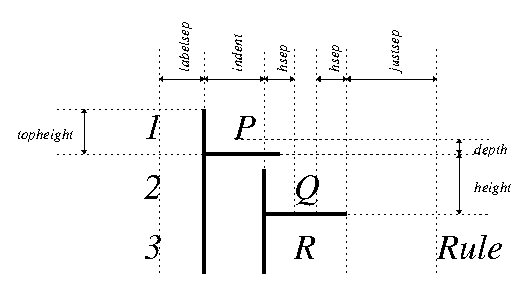
\includegraphics{fitchdoc1.eps}\]
The default dimensions are:
\[  \verb!\nddim{4.5ex}{3.5ex}{1.5ex}{1em}{1.6em}{.5em}{2.5em}{.2mm}!.
\]
In addition, there is a dimension called \verb!\ndindent!, controls
the amount of extra indentation used on continuation lines as
discussed in Section~\ref{subsec-continuation}. It can be changed and
is \verb!1ex!  by default.

\subsection{Other comments}

The goal was to design a flexible package which would not impose any
constraints on the form of derivations, while making typesetting easy.
With this package, it is in fact possible to typeset incomplete,
ill-formed, or invalid derivations. Sometimes it is pedagogically necessary
to do so.

There are no arbitrary limits on the size or nesting depth of a derivation,
except for the obvious requirement of fitting horizontally on the
printed page.

\section{Copyright and license}

The following notice applies to the \verb!fitch.sty! macros.

Copyright: {\copyright} 2002--2005 Peter Selinger

This program is free software; you can redistribute it and/or modify
it under the terms of the GNU General Public License as published by
the Free Software Foundation; either version 2, or (at your option)
any later version.

This program is distributed in the hope that it will be useful, but
WITHOUT ANY WARRANTY; without even the implied warranty of
MERCHANTABILITY or FITNESS FOR A PARTICULAR PURPOSE. See the GNU
General Public License for more details.

You should have received a copy of the GNU General Public License
along with this program; if not, write to the Free Software Foundation,
Inc., 59 Temple Place, Suite 330, Boston, MA 02111-1307, USA.

\end{document}
